\documentclass[final]{beamer}
\usepackage{grffile}
\mode<presentation>{\usetheme{I6pd2}}
\usepackage[english]{babel}
\usepackage[latin1]{inputenc}
\usecolortheme{wolverine}
\usepackage{amsmath,amsthm, amssymb, latexsym}
\usepackage[orientation=portrait,size=a0,scale=1.4,debug]{beamerposter}
\usepackage{array,booktabs,tabularx}
\newcolumntype{Z}{>{\centering\arraybackslash}X} 
\newcommand{\pphantom}{\textcolor{ta3aluminium}} 
\setbeamercolor{some beamer element}{fg=red}
\listfiles
\beamertemplateballitem
 
%%%%%%%%%%%%%%%%%%%%%%%%%%%%%%%%%%%%%%%%%%%%%%%%%%%%%%%%%%%%%%%%%%%%%%%%%%%%%%%%%%%%%%

\title{{\huge An Investigation into the Parameters of Photospheric Radius Expansion X-ray Bursts}}
\author{{\bf M. von Steinkirch, J. M. Lattimer, A. C. Calder}}
\institute[Stony Brook University]{Stony Brook University }
\newlength{\columnheight}
\setlength{\columnheight}{100cm}

%%%%%%%%%%%%%%%%%%%%%%%%%%%%%%%%%%%%%%%%%%%%%%%%%%%%%%%%%%%%%%%%%%%%%%%%%%%%%%%%%%%%%%


\begin{document}
\begin{frame}


%%%%%%%%%%%%%%%%%%%%%%%%%%%%%%%%%%%%%%%%%%%%%%%%%%%%%%%%%%%%%%%%%%%%%%%%%%%%%%%%%%%%%%

\begin{block}{Abstract}
The determination of the equation of state (EoS) of the cold ultradense matter in the core of neutron stars (NS) has been one of the biggest challenges of high-energy astrophysics. This EoS can be constrained if the NS masses and radii are determined from observational methods. For instance, these parameters can be obtained from certain X-ray bursting NS's; some of which can be strong enough to reach the Eddington luminosity and will exhibit photospheric radius expansion (PRE) bursts. These events give us insight into the underlying NS's compactness, which simultaneously leads to estimates of their masses and radii. At present, there is  disagreement over the interpretation of these bursts, resulting in relatively small or large radius estimates. An open question to be investigated is whether or not the touchdown is the moment when the photosphere coincides with the neutron star surface. We present preliminary results from studies on the PRE X-ray bursts aiming towards discerning and characterizing 
differences in the interpretation of these events. 
\end{block}


%%%%%%%%%%%%%%%%%%%%%%%%%%%%%%%%%%%%%%%%%%%%%%%%%%%%%%%%%%%%%%%%%%%%%%%%%%%%%%%%%%%%%%

\vskip3ex

%%%%%%%%%%%%%%%%%%%%%%%%%%%%%%%%%%%%%%%%%%%%%%%%%%%%%%%%%%%%%%%%%%%%%%%%%%%%%%%%%%%%%%

\begin{columns}


%%%%%%%%%%%%%%%%%%%%%%%%%%%%%%%%%%%%%%%%%%%%%%%%%%%%%%%%%%%%%%%%%%%%%%%%%%%%%%%%%%%%%%

\begin{column}{.49\textwidth}
\begin{beamercolorbox}[center,wd=\textwidth]{postercolumn}
\begin{minipage}[T]{.95\textwidth} 
\parbox[t][\columnheight]{\textwidth}
{ 

%%%%%%%%%%%%%%%%%%%%%%%%%%%%%%%%%%%%%%%%%%%%%%%%%%%%%%%%%%%%%%%%%%%%%%%%%%%%%%%%%%%%%%

\begin{block}{What are X-ray Bursters?}

\begin{itemize}
 \item More than {\bf 2000 neutron stars} have been discovered, from pulsating sources in radio to bright persistent sources in X-rays \cite{01}.
 
 \vskip2ex
 
 
\item There is  evidence of neutron star surface emission from {\bf thermonuclear X-ray bursters} ({\bf Type I X-Ray Bursters, XRB}) in {\bf low-mass X-ray binaries (LMXB)}. These sources can put constraints on the {\bf neutron star (cold dense matter) equation of state} \cite{02}.

\vskip2ex



\item Observations of neutron stars during thermonuclear bursts have led to the {\bf first constraining measurements of neutron star radii}: 9 km $<$ R $<$ 12 km \cite{1}.

\end{itemize}              

\end{block}

%%%%%%%%%%%%%%%%%%%%%%%%%%%%%%%%%%%%%%%%%%%%%%%%%%%%%%%%%%%%%%%%%%%%%%%%%%%%%%%%%%%%%%

\vskip3ex

%%%%%%%%%%%%%%%%%%%%%%%%%%%%%%%%%%%%%%%%%%%%%%%%%%%%%%%%%%%%%%%%%%%%%%%%%%%%%%%%%%%%%%

\begin{block}{The Photospheric Radius Expansion during  X-ray Bursts}   

\begin{itemize}
\item  Observations of neutron stars come from the outermost layer, the {\bf photosphere}, which is in radioactive equilibrium given by a flux, $$F=\sigma_{\rm S}T^4_{\rm eff},$$
where $\sigma_{\rm S}$ is the Stefan's constant and $T_{eff}$ is the {\bf effective temperature} at the surface.

\vskip2ex

\item {\bf Photospheric Radius Expansion bursts} are a {\bf very bright} subset of thermonuclear X-ray bursts. After the radius expansion, the moment when the photosphere returns to the neutron star radius is called {\bf touchdown point}. 

\vskip2ex

\item A first attempt to extract the neutron stars masses and radii was by identifying the moment of touchdown to the moment when the atmosphere reaches the {\bf Eddington (luminosity) limit},
$$L_{\rm Edd} = 4 \pi R^2 \sigma_{\rm T} T^4_{\rm eff}.$$

\vskip2ex

\item This approach is not accurate enough and {\bf further refinement of the results of the ref. \cite{1} for the equation of states of the cold dense matter depends on better atmosphere modeling}.


\vskip2ex

\item Realistically, the {\bf spectra of the neutron star's atmosphere} look likes a {\bf black-body function}, but {\bf shifted to higher temperatures} by a {\bf color correction factor},

$$f_{\rm c} = \frac{T_{\rm c}}{T_{\rm eff}}.$$

\vskip2ex

\end{itemize}
\end{block}


%%%%%%%%%%%%%%%%%%%%%%%%%%%%%%%%%%%%%%%%%%%%%%%%%%%%%%%%%%%%%%%%%%%%%%%%%%%%%%%%%%%%%%

\vskip3ex


%%%%%%%%%%%%%%%%%%%%%%%%%%%%%%%%%%%%%%%%%%%%%%%%%%%%%%%%%%%%%%%%%%%%%%%%%%%%%%%%%%%%%%

\begin{block}{References}
\begin{thebibliography}{}
{\small
\bibitem{01}[1] T. Strohmayer $\&$ L. Bildsten, {\it \small New Views of Thermonuclear Bursts}, 2003.
\bibitem{02}[2]  L. Bildsten, {\it \small Theory and Observation of Type I X-Ray Bursts from Neutron Stars}, 2000.
\bibitem{1}[3] A. W. Steiner et al, {\it \small The Equation of State from Observed Masses and Radii of Neutron Stars}, 2010.
\bibitem{5}[4] V. Suleimanov et al, {\it \small X-ray Bursting Neutron Star
Atmosphere Models}, 2010.
\bibitem{6}[5] Models simulated by Zach Medin (work in progress), 2012. 

}
\end{thebibliography}
 \end{block}


%%%%%%%%%%%%%%%%%%%%%%%%%%%%%%%%%%%%%%%%%%%%%%%%%%%%%%%%%%%%%%%%%%%%%%%%%%%%%%%%%%%%%%

\vskip3ex



%%%%%%%%%%%%%%%%%%%%%%%%%%%%%%%%%%%%%%%%%%%%%%%%%%%%%%%%%%%%%%%%%%%%%%%%%%%%%%%%%%%%%%


\begin{block}{Acknowledgments}
This work was supported in part by the DOE under grant DE-FG02-87ER40317. We acknowledge and thank to  Zach Medin and Chris Fryer for providing the data and for assisting the development of this work.
\end{block}


}
  

%%%%%%%%%%%%%%%%%%%%%%%%%%%%%%%%%%%%%%%%%%%%%%%%%%%%%%%%%%%%%%%%%%%%%%%%%%%%%%%%%%%%%%

\end{minipage}
\end{beamercolorbox}
\end{column}

%%%%%%%%%%%%%%%%%%%%%%%%%%%%%%%%%%%%%%%%%%%%%%%%%%%%%%%%%%%%%%%%%%%%%%%%%%%%%%%%%%%%%%



\begin{column}{.49\textwidth}
      \begin{beamercolorbox}[center,wd=\textwidth]{postercolumn}
        \begin{minipage}[T]{.95\textwidth} % tweaks the width, makes a new \textwidth
          \parbox[t][\columnheight]{\textwidth}
{



\begin{block}{Atmospheric Simulations of Thermonuclear X-ray Bursters }

\begin{itemize}
\item Simulations of {\bf  models for the Neutron Star's atmosphere} provide the {\bf spectrum and pattern of radiation} from their crusts and cores.

\vskip2ex

\item The {\bf basic assumptions} for these simulations are {\bf plane-parallel geometry}, {\bf radioactive equilibrium}, and {\bf hydro-static equilibrium}.

\vskip2ex


\item Many {\bf  different physical parameters} are considered in these models: different {\bf chemical compositions} ({\it e.g.}, the hydrogen fraction, $X$),  {\bf gravitational acceleration at surface} ($g$),  {\bf magnetic field strengths}, and  {\bf temperature at the surface} ($T_{eff}$).


\end{itemize}

\end{block}

%%%%%%%%%%%%%%%%%%%%%%%%%%%%%%%%%%%%%%%%%%%%%%%%%%%%%%%%%%%%%%%%%%%%%%%%%%%%%%%%%%%%%%

\vskip3ex

%%%%%%%%%%%%%%%%%%%%%%%%%%%%%%%%%%%%%%%%%%%%%%%%%%%%%%%%%%%%%%%%%%%%%%%%%%%%%%%%%%%%%%


\begin{block}{Preliminary Results on  Atmospheric Modeling and Spectra Fitting }

Our study begins by fitting a diluted black-body spectrum to existing
models \cite{5} \cite{6} to verify our method. We have fitted these data to a black-body spectrum in five different ways, with $f_{\rm c}$ as one of the parameters. 


  \begin{columns}
\begin{column}{0.7\textwidth} 

\quad

\begin{center}
		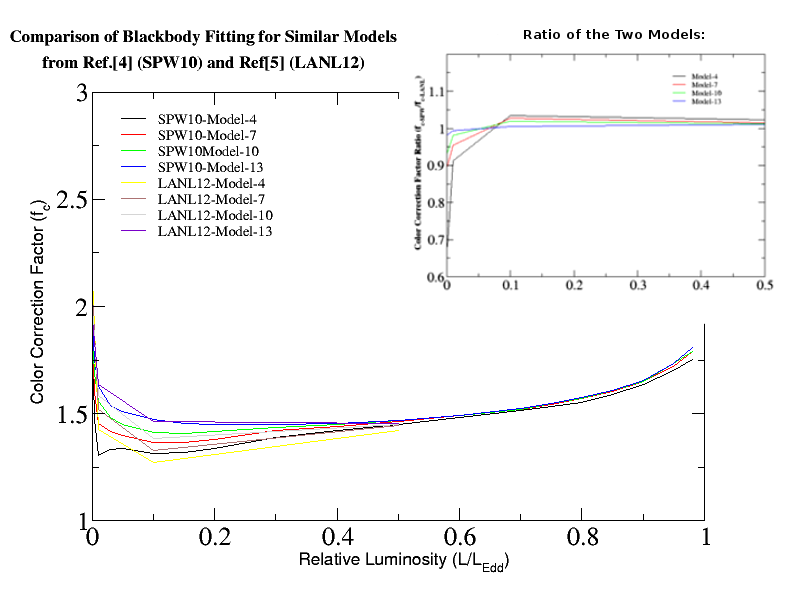
\includegraphics[width=0.95\linewidth]{models.png}
		\end{center}
  \end{column}
\begin{column}{0.3\textwidth} 

{\scriptsize All the displayed models have $\log g = 14.0$ with the following parameters:}

\quad

 	\begin{itemize}
 	\item {\scriptsize model 4: $X=0.74$, $Z=Z_{\odot}$,}
 	\item {\scriptsize model 7: $X=0.74$, $Z=0.30Z_{\odot}$,}
 	\item {\scriptsize model 10: $X=1$, $Z=0.1Z_{\odot}$,}
 	\item {\scriptsize model 13: $X=1$, $Z=0.01Z_{\odot}$.}  	
	\end{itemize}

  \end{column}
  \end{columns}
  
  \quad
  
  \begin{center}  
   	{\scriptsize Comparison of all the four fitting modules for  model 4 and module 13:}
  \end{center}
  
  \begin{columns}
\begin{column}{0.5\textwidth} 
\begin{center}
		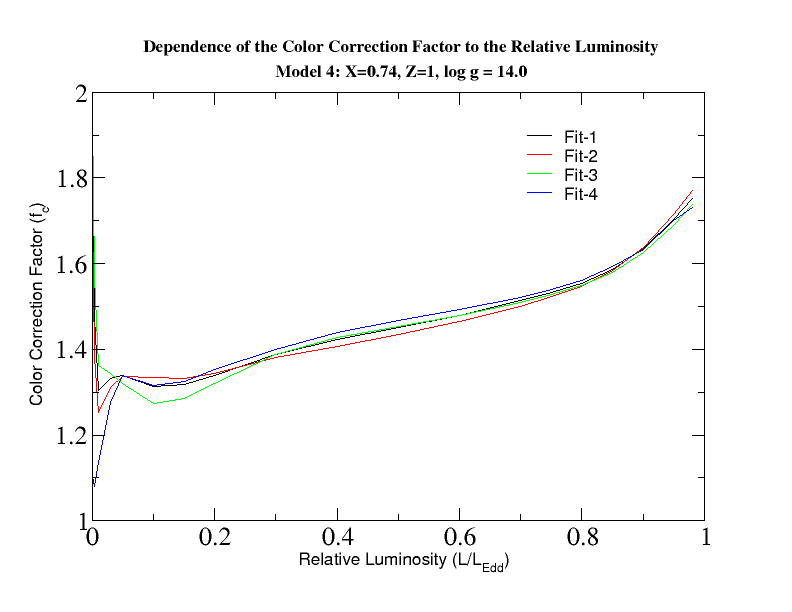
\includegraphics[width=0.98\linewidth]{all-fits2.png}
		\end{center}
  \end{column}
\begin{column}{0.5\textwidth} 
		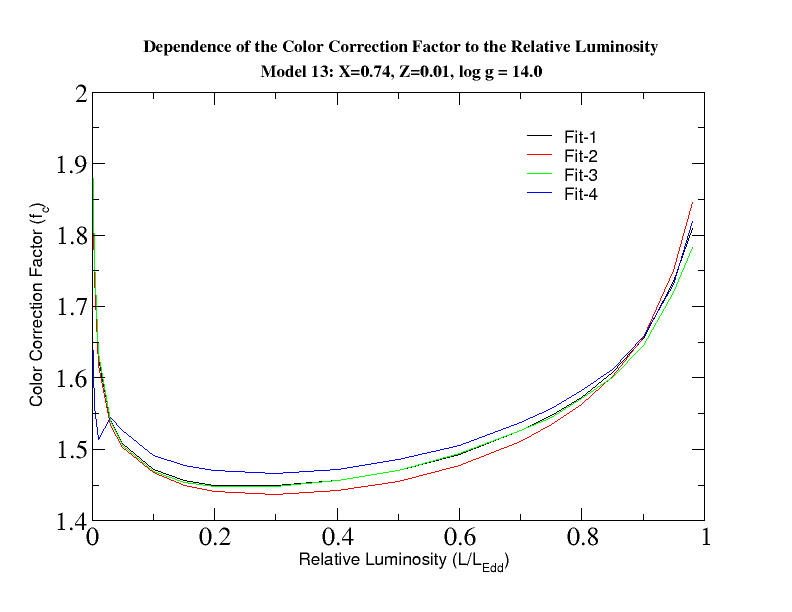
\includegraphics[width=0.98\linewidth]{all-fits.png}
  \end{column}
  \end{columns}  



\end{block}

%%%%%%%%%%%%%%%%%%%%%%%%%%%%%%%%%%%%%%%%%%%%%%%%%%%%%%%%%%%%%%%%%%%%%%%%%%%%%%%%%%%%%%


\vskip3ex

%%%%%%%%%%%%%%%%%%%%%%%%%%%%%%%%%%%%%%%%%%%%%%%%%%%%%%%%%%%%%%%%%%%%%%%%%%%%%%%%%%%%%%



\begin{block}{Discussion Conclusions}
\begin{itemize}
\item  X-ray bursts are an useful tool for inferring {\bf neutron stars masses and radii}. However, systematic and statistical errors currently do not allow us to pin down a {\bf unique equation of state of the cold ultra-dense matter}. 

\vskip2ex

\item  We have developed and tested a {\bf module for fitting a diluted black-body spectra to simulations of photospheric X-ray bursts}.
\vskip2ex

\item With this verified technique, we will  {\bf explore parameters and new models} to determine {\bf masses and radii of neutron stars} from observed {\bf X-ray bursts} and further constrain the {\bf equations of state}.


\end{itemize}
\end{block}


%%%%%%%%%%%%%%%%%%%%%%%%%%%%%%%%%%%%%%%%%%%%%%%%%%%%%%%%%%%%%%%%%%%%%%%%%%%%%%%%%%%%%%

\vskip3ex





%%%%%%%%%%%%%%%%%%%%%%%%%%%%%%%%%%%%%%%%%%%%%%%%%%%%%%%%%%%%%%%%%%%%%%%%%%%%%%%%%%%%%%


}
  

%%%%%%%%%%%%%%%%%%%%%%%%%%%%%%%%%%%%%%%%%%%%%%%%%%%%%%%%%%%%%%%%%%%%%%%%%%%%%%%%%%%%%%

\end{minipage}
\end{beamercolorbox}
\end{column}


%%%%%%%%%%%%%%%%%%%%%%%%%%%%%%%%%%%%%%%%%%%%%%%%%%%%%%%%%%%%%%%%%%%%%%%%%%%%%%%%%%%%%%

\end{columns}

%%%%%%%%%%%%%%%%%%%%%%%%%%%%%%%%%%%%%%%%%%%%%%%%%%%%%%%%%%%%%%%%%%%%%%%%%%%%%%%%%%%%%%

\end{frame}
\end{document}
